\documentclass{bredelebeamer}

%%%%%%%%%%%%%%%%%%%%%%%%%%%%%%%%%%%%%%%%%%%%%%%%

\title[Programación en MatLAB]{Introducción a la programación con MatLAB}
\subtitle{Módulo 04 - Operaciones vectoriales (introducción)}

\author{Autor1 - Autor2 - Autor3\inst{1}}
\institute[UTN.BA]
{
  \inst{1}%
  Universidad Tecnológica Nacional\\
  Facultad Regional Buenos Aires
  }

\date{dia agosto 2018}

\subject{Taller de programación}

\logo{

\includegraphics[scale=0.15]{images/logo.png}
}

%%%%%%%%%%%%%%%%%%%%%%%%%%%%%%%%%%%%%%%%%%%%%%%%%%%%%%%%%%%%%%%%%%%%%
\begin{document}

\begin{frame}
  \titlepage 
\end{frame}

%%%%%%%%%%%%%%%%%%%%%%%%%%%%%%%%%%%%%%%%%%%%%%%%%%%%%%%%%%%%%%%%%%%%%

% Sección de operaciones vectoriales

%%%%%%%%%%%%%%%%%%%%%%%%%%%%%%%%%%%%%%%%%%%%%%%%%%%%%%%%%%%%%%%%%%%%%

\section{Operaciones vectoriales}

\begin{frame}{Tipos de operaciones}
Existen dos tipos de operaciones aritméticas: las operaciones aritméticas matriciales, que se rigen por las reglas del álgebra lineal, y las operaciones aritméticas con vectores, que se realizan elemento a elemento.\\
\begin{enumerate}
\item Las operaciones matemáticas simples entre escalares y vectores aplican el escalar a todos los elementos del vector según la operación definida.
\item Las operaciones simples entre vectores se realizan elemento a elemento.
\end{enumerate}
\end{frame}

\begin{frame}{Tipos de operaciones}
\begin{table}[]
\centering
\begin{tabular}{|c|c|}
\hline
\multicolumn{2}{|c|}{a=\{a1,a2,...,an\}, b=\{b1,b2,...,bn\} c=escalar}                                                                           \\ \hline
a+c={[}a1+c a2+c...,an+c{]}                                                                            & Suma de un escalar y un vector          \\ \hline
a*c={[}a1*c a2*c ... an*c{]}                                                                           & Producto de un escalar por un vector    \\ \hline
a + b = {[} a1+b1 a2+b2 ... an+bn{]}                                                                   & Suma de dos vectores                    \\ \hline
a. * b = {[} a1*b1 a2*b2 ... an*bn{]}                                                                  & Producto de dos vectores                \\ \hline
a. / b = {[} a1/b1 a2/b2 ... an/bn{]}                                                                  & Cociente a la derecha de dos vectores   \\ \hline
a. \textbackslash b = {[} a1\textbackslash{}b1 a2\textbackslash{}b2 ... an\textbackslash{}bn{]}        & Cociente a la izquierda de dos vectores \\ \hline
a.\textasciicircum{}c = {[}a1\textasciicircum{}c a2\textasciicircum{}c ... an\textasciicircum{}c{]}    & Vector elevado a escalar                \\ \hline
c.\textasciicircum{}a = {[}c\textasciicircum{}a1 c\textasciicircum{}a2 ... c\textasciicircum{}an{]}    & Escalar elevado a vector                \\ \hline
a.\textasciicircum{}b = {[}a1\textasciicircum{}b1 a2\textasciicircum{}b2 ... an\textasciicircum{}bn{]} & Vector elevado a vector                 \\ \hline
\end{tabular}
\end{table}
\begin{alertblock}{Tener en cuenta}
Hay que tener presente que los vectores han de ser de la misma longitud y que en el producto, cociente y potencia el primer operando va seguido de un punto.
\end{alertblock}
\end{frame}

\begin{frame}{Ejercicio práctico 5}
\begin{enumerate}
\item Defina la matriz a = [2.3 5.8 9] como una variable
\item Sume 3 a cada elemento en a
\item Defina la matriz b = [5.2 3.14 2] como una variable matlab
\item Sume cada elemento de la matriz a y la matriz b
\item Multiplique cada elemento en a por el correspondiente elemento en b
\item Eleve al cuadrado cada elemento en la matriz a
\item Cree una matriz llamada c de valores igualmente espaciados, desde 0 hasta 10, con un incremento de 1
\item Cree una matriz llamada d de valores igualmente espaciados, desde 0 hasta 10, con un incremento de 2.
\item Use la función linspace para crear una matriz de seis valores igualmente espaciados, desde 10 hasta 20.
\item Use la función logspace para crear una matriz de cinco valores logarítmicamente espaciados entre 10 y 100
\end{enumerate}
\end{frame}

%%%%%%%%%%%%%%%%%%%%%%%%%%%%%%%%%%%%%%%%%%%%%%%%%%%%%%%%%%%%%%%%%%%%%

% Sección de consultas

%%%%%%%%%%%%%%%%%%%%%%%%%%%%%%%%%%%%%%%%%%%%%%%%%%%%%%%%%%%%%%%%%%%%%

\section{Consultas}
\begin{frame}{Consultas}
\begin{center}

\includegraphics[scale=0.3]{images/consultas.png}
\end{center}
\end{frame}


%%%%%%%%%%%%%%%%%%%%%%%%%%%%%%%%%%%%%%%%%%%%%%%%%%%%%%%%%%%%%%%%%%%%%

% Sección de bibliografía

%%%%%%%%%%%%%%%%%%%%%%%%%%%%%%%%%%%%%%%%%%%%%%%%%%%%%%%%%%%%%%%%%%%%%

\section{Bibliografia}

\begin{frame}{Bibliografía}
\begin{columns}
\begin{column}{0.5\textwidth}
\begin{center}

\includegraphics[scale=0.4]{images/biblio1.png}
\end{center}
\end{column}
\begin{column}{0.5\textwidth}
\begin{center}
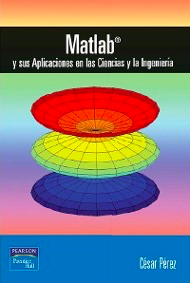
\includegraphics[scale=0.5]{images/biblio2.png}
\end{center}
\end{column}
\end{columns}
\end{frame}

\end{document}
